\documentclass[useAMS,usenatbib,referee]{biom}
%\documentclass[useAMS,usenatbib,referee]{biom}
%
%
%  Papers submitted to Biometrics should ALWAYS be prepared
%  using the referee option!!!!
%
%
% If your system does not have the AMS fonts version 2.0 installed, then
% remove the useAMS option.
%
% useAMS allows you to obtain upright Greek characters.
% e.g. \umu, \upi etc.  See the section on "Upright Greek characters" in
% this guide for further information.
%
% If you are using AMS 2.0 fonts, bold math letters/symbols are available
% at a larger range of sizes for NFSS release 1 and 2 (using \boldmath or
% preferably \bmath).
%
% The usenatbib command allows the use of Patrick Daly's natbib package for
% cross-referencing.
%
% If you wish to typeset the paper in Times font (if you do not have the
% PostScript Type 1 Computer Modern fonts you will need to do this to get
% smoother fonts in a PDF file) then uncomment the next line
% \usepackage{Times}
%%%%% AUTHORS - PLACE YOUR OWN MACROS HERE %%%%%

\usepackage[figuresright]{rotating}
\usepackage{tikz}
\usepackage{amsmath}
\usepackage[hyphens]{url} % not crucial - just used below for the URL
\usepackage{hyperref}
\usepackage[utf8]{inputenc}
\usepackage{graphicx}
\usepackage{longtable}
\usepackage{booktabs}
%% \raggedbottom % To avoid glue in typesetteing, sbs>>


% tightlist command for lists without linebreak
\providecommand{\tightlist}{%
  \setlength{\itemsep}{0pt}\setlength{\parskip}{0pt}}

% From pandoc table feature
\usepackage{longtable,booktabs,array}
\usepackage{calc} % for calculating minipage widths
% Correct order of tables after \paragraph or \subparagraph
\usepackage{etoolbox}
\makeatletter
\patchcmd\longtable{\par}{\if@noskipsec\mbox{}\fi\par}{}{}
\makeatother
% Allow footnotes in longtable head/foot
\IfFileExists{footnotehyper.sty}{\usepackage{footnotehyper}}{\usepackage{footnote}}
\makesavenoteenv{longtable}


%%%%%%%%%%%%%%%%%%%%%%%%%%%%%%%%%%%%%%%%%%%%%%%%

\setcounter{footnote}{2}

\title[]{Average treatment effect of cholesterol-lowering medication and
average systolic blood pressure (SBP), mm Hg.}

\author{ Jackson
Gazin \email{\href{mailto:gazij22@wfu.edu}{\nolinkurl{gazij22@wfu.edu}}} \\ Department
of Statistics, Wake Forest University  \and
		 Ashley
Mullan \email{\href{mailto:mullae22@wfu.edu}{\nolinkurl{mullae22@wfu.edu}}} \\ Department
of Statistics, Wake Forest University  \and
		 Anh
Nguyen \email{\href{mailto:nguyp22@wfu.edu}{\nolinkurl{nguyp22@wfu.edu}}} \\ Department
of Statistics, Wake Forest University 
	   }


\begin{document}


\date{{\it Received Dec} 2023}

\pagerange{\pageref{firstpage}--\pageref{lastpage}} \pubyear{2023}

\volume{0}
\artmonth{January}
\doi{0000-0000-0000}

%  This label and the label ``lastpage'' are used by the \pagerange
%  command above to give the page range for the article

\label{firstpage}

%  pub the summary here

\begin{abstract}
We investigate the average treatment effect among the treated (ATT) of
cholesterol-lowering medication on the mean systolic blood pressure (mm
Hg). Using data from the National Health and Nutrition Examination
Survey (NHANES), we use the Inverse Probability Weighting method to
estimate the ATT among adults living in the United States of America.
\end{abstract}

%
%  Please place your key words in alphabetical order, separated
%  by semicolons, with the first letter of the first word capitalized,
%  and a period at the end of the list.
%

\begin{keywords}
cholesterol-lowering medication,systolic blood pressure,blood pressure
control.
\end{keywords}

\maketitle

\hypertarget{intro}{%
\section{Introduction}\label{intro}}

Controlling blood pressure (BP) reduces the risk for cardiovascular
disease. However, the prevalence of BP control (i.e., systolic BP
\textless{} 140 mmHg and diastolic BP \textless{} 90 mmHg) among US
adults with hypertension has decreased \citep{cdc_prevalence_nodate}. In
2017-2018, prevalence of hypertension in the USA was 49.64\% while the
prevalence of blood control by medication is only 39.64\%
\citep{chobufo_prevalence_2020}. Further interventions are needed to
help improve the prevalence and hypertension control rates in the USA.

High blood pressure and high cholesterol often occur at the same time.
According to survey, 60.7\% to 64.3\% of people with high blood pressure
also have high cholesterol \citep{egan_blood_2013}. The prescription of
both anti-hypertensive and cholesterol-lowering drugs is generally
required for these patients. It is recommended that doctors prescribe
statin drugs like atorvastatin (Lipitor), and simvastatin (Zocor,
FloLipid) for patients with high cholesterol or patients with high blood
pressure (with or without high cholesterol)
\citep{williams_facing_2020}.

Statins (a chemical in cholesterol-lowering medication) have been proven
to minimize the risk of cardiovascular adverse events since it block a
substance the liver needs to make cholesterol \citep{liu_statins_2023}.
Thus statins have the potential to lower blood pressure. In many cases,
simultaneously lower blood pressure and cholesterol level
\citep{strazzullo_statins_2007}.

Using a causal analysis approach, we aim to explore whether taking
cholesterol-lowering medication have the potential to lower blood
pressure. By analyzing the publicly available National Health and
Nutrition Examination Survey (NHANES), we will estimate the average
treatment effect of taking cholesterol-lowing medication among those who
take the medication. Our exposure is whether or not a person has been
taking any cholesterol-loweing medication at the time of the survey. Our
primary outcome is the mean systolic blood pressure (DBP) at the time of
the survey. The average treatment effect among the treated (ATT) is the
estimand of the different in DBP between taking cholesterol-lowering
medication and not taking the medication. This estimand is conditioned
on the exposed group.

With this causal question in mind, we want to control for demographics
and a person bmi since high blood pressure disproportionately affect
men, people of color, older people, obese people and people with
diabetes and chronic kidney disease \citep{chobufo_prevalence_2020}.
Moreover, as stated before, if a patient have high BP, they are
sometimes prescribed cholesterol-lowering medication along with
anti-hypertensive medication to control for BP \citep{egan_blood_2013}.
In addition, if a person has high cholesterol, this has been shown to
cause increase in BP. Moreover, smoking has been shown to increase BP.
Furthermore, a person's BMI, smoking habit, and cholesterol may be a
result of poor lifestyle habit. There are distinct cluster of lifestyle
in different demographics. Patients with high BMI are also at risk of
having high cholesterol.

\hypertarget{methods}{%
\section{Materials and methods}\label{methods}}

\hypertarget{data}{%
\subsection{Data}\label{data}}

The National Health and Nutrition Examination Survey (NHANES) combines
interviews and physical examinations to assess the health and
nutritional status of adults and children in the United States of
America. The program started in the early 1960s and has been conducted
every two years since 1999. The survey samples from a nationally
representative 5,000 persons each year. The participants are located in
counties across the country, 15 of which are visited each year. The
interview asks questions about demographic, socioeconomic, dietary, and
health-related questions. The examination consists of medical, dental,
physiological measurements, and laboratory tests.

The NHANES dataset we are using is from the cardioStatsUSA R package.
The dataset contains information from the survey from 1999 to 2020 with
a sample of 59,799 rows and 111 chosen columns focusing on
cardiovascular disease. Each row is a noninstitutionalized US adults who
participated in the survey between 1999 and 2020. The columns contain
information about demographics, blood pressure levels, hypertension
status, antihypertensive medication usage, and co-morbidities.

For this analysis, we had 38977 rows with NA values. We decided to deal
with this by removing all the na values. We decided this was preferable
to removing certain columns since we were still left with 20,822 data
points which is still an extremely large data set. We also selected
columns that represent our treatment, our outcome out interest, and the
covariates we need to adjust for given the proposed causal directed
acyclic graph in the \protect\hyperlink{dags}{Causal directed acyclic
graphs} section

\hypertarget{exploratory-data-analysis}{%
\subsubsection{Exploratory data
analysis}\label{exploratory-data-analysis}}

\begin{figure}
\centering
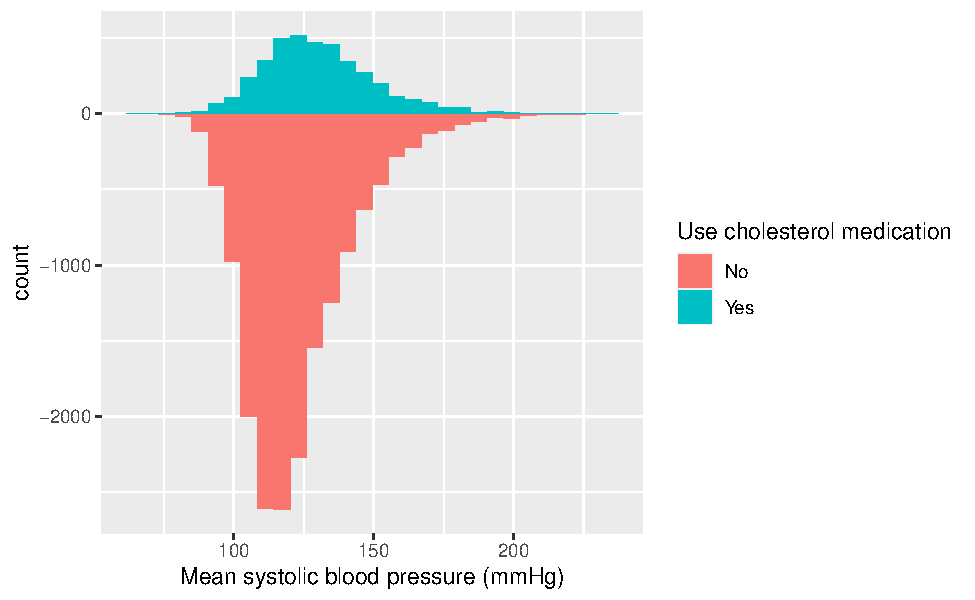
\includegraphics{final-project_files/figure-latex/fig_eda-1.pdf}
\caption{Mirror histogram by whether the participants use cholesterol
medication}
\end{figure}

\hypertarget{dags}{%
\subsubsection{Causal directed acyclic graphs}\label{dags}}

We visualize the assumptions that we're making about the causal
relationships between the use of cholesterol-lowering medication (the
exposure), the mean systolic blood pressure (the outcome), and other
possible confounders in the data set using a directed acyclic graph
(DAG) (Figure @ref(fig:fig-dag)). The demographic variable include: age,
gender, and race.

\begin{figure}
\centering
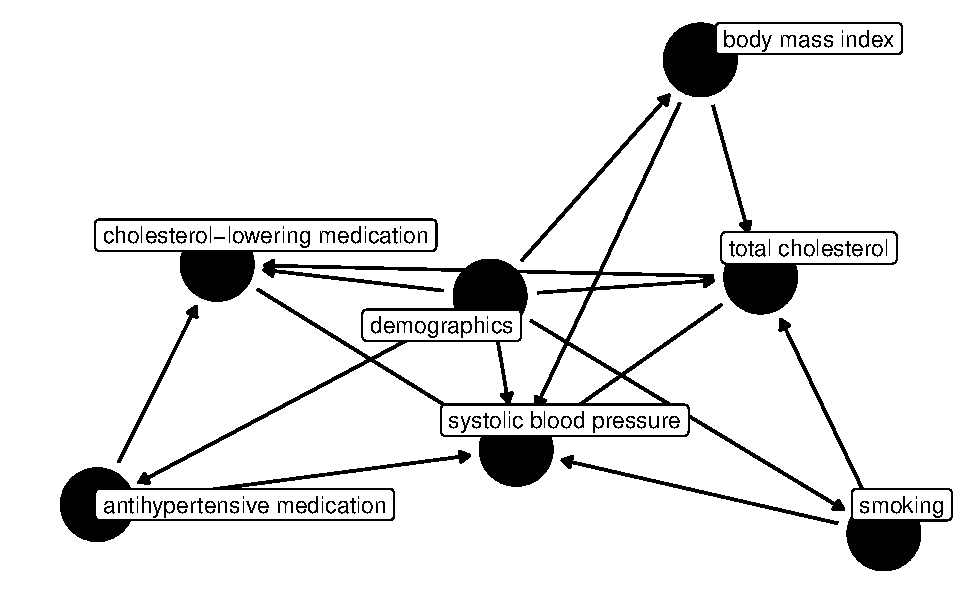
\includegraphics{final-project_files/figure-latex/fig-dag-1.pdf}
\caption{Causal direct acyclic graph between cholesterol-lowering
medication and the mean systolic blood pressure}
\end{figure}

Given our assumptions, we obtained the adjustment set that will help us
control for possible confounders (@ref(fig:fig\_adjustment)). Our
adjustment set only includes the amount of total cholesterol,
demographics, and whether they use anti-hypertensive medication.

\begin{figure}
\centering
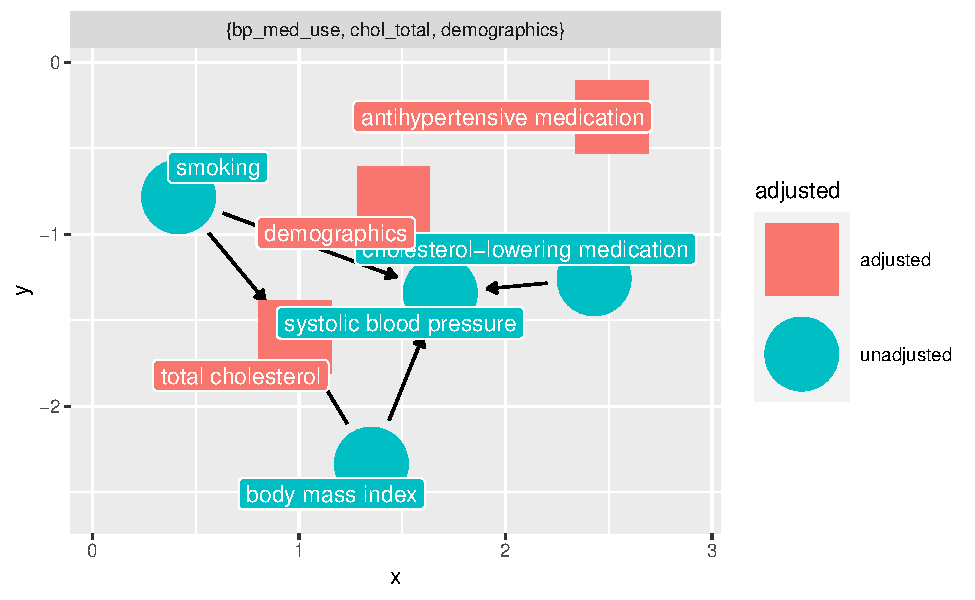
\includegraphics{final-project_files/figure-latex/fig_adjustment-1.pdf}
\caption{Causal adjustment set}
\end{figure}

\hypertarget{statistical-methods}{%
\subsection{Statistical methods}\label{statistical-methods}}

We aim to answer our causal question by fitting an average treatment
effect among the treated. Our causal question is as follows: Among those
who take cholesterol lowering medication, does taking this cholesterol
lowering medication change their systolic blood pressure?

We fitted a propensity score model with our DAGS adjustment set as our
explanatory variable (\protect\hyperlink{dags}{Causal directed acyclic
graphs}), and whether a person was taking cholesterol medication as our
response variable. We employed a logistic regression model for the
propensity score model. We log transform our age variable since the
distribution is usually skewed.

Subsequently, we used the propensity score as weight for our exposure
variable (taking cholesterol medication). To estimate the average
treatment effect among the treated, we fit a weighted linear regression
model. We use the weighted cholesterol medication as our explanatory
variable and systolic blood pressure as our response variable.

To assess the appropriateness of our propensity score model and proceed
with our final model, we perform diagnostic using weighted mirrored
histograms, empirical cumulative distribution function (ECDF) plots, and
Love plots.

\hypertarget{results}{%
\section{Results}\label{results}}

\hypertarget{study-population}{%
\subsection{Study population}\label{study-population}}

\begin{longtable}[]{@{}
  >{\raggedright\arraybackslash}p{(\columnwidth - 6\tabcolsep) * \real{0.4348}}
  >{\centering\arraybackslash}p{(\columnwidth - 6\tabcolsep) * \real{0.1739}}
  >{\centering\arraybackslash}p{(\columnwidth - 6\tabcolsep) * \real{0.1739}}
  >{\centering\arraybackslash}p{(\columnwidth - 6\tabcolsep) * \real{0.2174}}@{}}
\caption{\textbf{Table 1. Survey Participant
Characteristics}}\tabularnewline
\toprule()
\begin{minipage}[b]{\linewidth}\raggedright
\textbf{Taking Cholesterol-lowering Medication}
\end{minipage} & \begin{minipage}[b]{\linewidth}\centering
\textbf{No}, N = 21,071
\end{minipage} & \begin{minipage}[b]{\linewidth}\centering
\textbf{Yes}, N = 4,433
\end{minipage} & \begin{minipage}[b]{\linewidth}\centering
\textbf{Overall}, N = 25,504
\end{minipage} \\
\midrule()
\endfirsthead
\toprule()
\begin{minipage}[b]{\linewidth}\raggedright
\textbf{Taking Cholesterol-lowering Medication}
\end{minipage} & \begin{minipage}[b]{\linewidth}\centering
\textbf{No}, N = 21,071
\end{minipage} & \begin{minipage}[b]{\linewidth}\centering
\textbf{Yes}, N = 4,433
\end{minipage} & \begin{minipage}[b]{\linewidth}\centering
\textbf{Overall}, N = 25,504
\end{minipage} \\
\midrule()
\endhead
\textbf{Total cholesterol, mg/dL} & 192 (166, 221) & 173 (149, 201) &
189 (163, 218) \\
Unknown & 237 & 64 & 301 \\
\textbf{Systolic blood pressure (SBP), mm Hg} & 119 (109, 131) & 129
(117, 142) & 120 (110, 133) \\
Unknown & 914 & 171 & 1,085 \\
\textbf{Race/ethnicity} & & & \\
Non-Hispanic White & 8,639 (41\%) & 2,320 (52\%) & 10,959 (43\%) \\
Non-Hispanic Black & 4,430 (21\%) & 840 (19\%) & 5,270 (21\%) \\
Non-Hispanic Asian & 1,179 (5.6\%) & 244 (5.5\%) & 1,423 (5.6\%) \\
Hispanic & 5,973 (28\%) & 865 (20\%) & 6,838 (27\%) \\
Other & 850 (4.0\%) & 164 (3.7\%) & 1,014 (4.0\%) \\
\textbf{Gender} & & & \\
Men & 9,943 (47\%) & 2,356 (53\%) & 12,299 (48\%) \\
Women & 11,128 (53\%) & 2,077 (47\%) & 13,205 (52\%) \\
\textbf{Age at Screening Adjudicated - Recode} & 42 (28, 58) & 66 (58,
75) & 47 (31, 63) \\
\textbf{Self-reported antihypertensive medication use} & 3,475 (17\%) &
2,880 (65\%) & 6,355 (25\%) \\
Unknown & 116 & 4 & 120 \\
\bottomrule()
\end{longtable}

\hypertarget{propensity-score-model-and-diagnostics}{%
\subsection{Propensity score model and
Diagnostics}\label{propensity-score-model-and-diagnostics}}

We fitted a propensity score model with ``total cholesterol'' in mg/dL
as our explanatory variable and ``taking cholesterol medication'' as our
response variable. We employed a Logistic Regression model for this
purpose. Subsequently, we examined a Mirrored Histogram of our
propensity scores for both exposure groups. The table below demonstrates
significant overlap in propensity scores across both groups, indicating
very little evidence of a positivity violation in our model, which is
promising.

Next, we used our propensity score model to generate weights for the
average treatment effect among the treated (ATT), aligning with our
causal question. To assess the appropriateness of our propensity score
model and the resulting weights, we created a Weighted Mirror Histogram
of our propensity scores. As shown below, we achieved sufficient balance
between the exposed and unexposed groups. Furthermore, the distribution
of the unexposed group now resembles that of the exposed group, which is
the desired outcome when using ATT weights.

We also generated a love plot, displaying the standardized mean
difference changes for the exposed and unexposed groups regarding our
``total cholesterol'' variable in both unweighted and weighted data. As
expected, our weighted data exhibit a standardized mean difference of 0
for the ``total cholesterol'' variable, which is ideal and allows us to
proceed.

Finally, we created a weighted empirical cumulative distribution
function (eCDF) plot for our continuous variable, ``total cholesterol.''
As shown below, the Weighted ECDF plot indicates balance not only in the
mean across exposure groups but also across their respective
distributions. No changes are required for our model, and we can now
proceed to estimate our average treatment effect among the treated.

\hypertarget{diagnostics}{%
\subsubsection{Diagnostics}\label{diagnostics}}

\begin{figure}
\centering
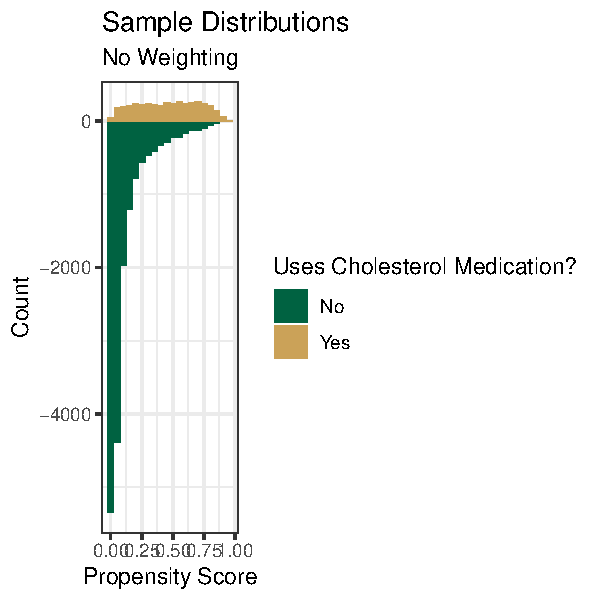
\includegraphics{final-project_files/figure-latex/fig_diag1-1.pdf}
\caption{Mirror histogram of propensity score by treatment group}
\end{figure}

\begin{figure}
\centering
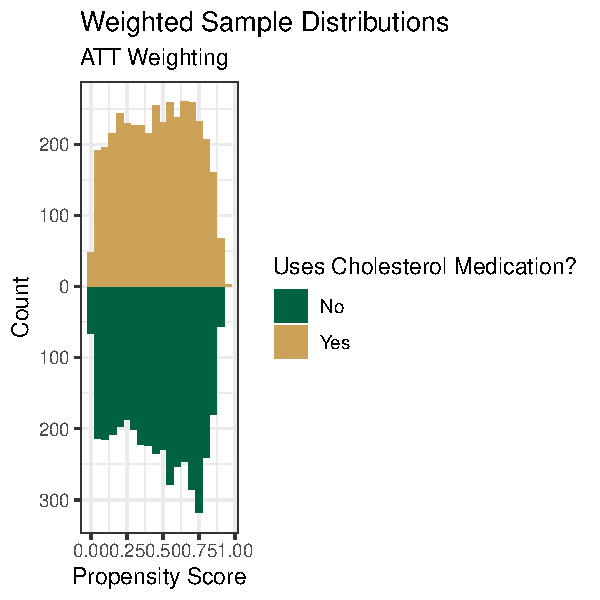
\includegraphics{final-project_files/figure-latex/fig_diag2-1.pdf}
\caption{Mirror histogram by whether the participants use cholesterol
medication using ATT weighting}
\end{figure}

\begin{figure}
\centering
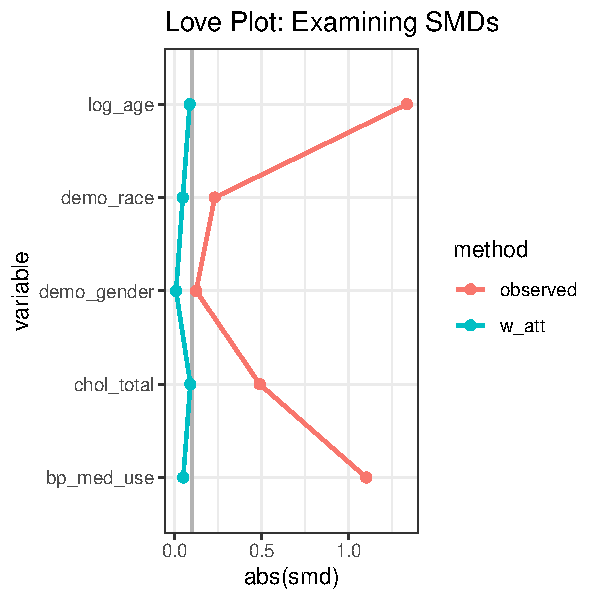
\includegraphics{final-project_files/figure-latex/fig_love-1.pdf}
\caption{Love plot for covariates}
\end{figure}

\begin{figure}
\centering
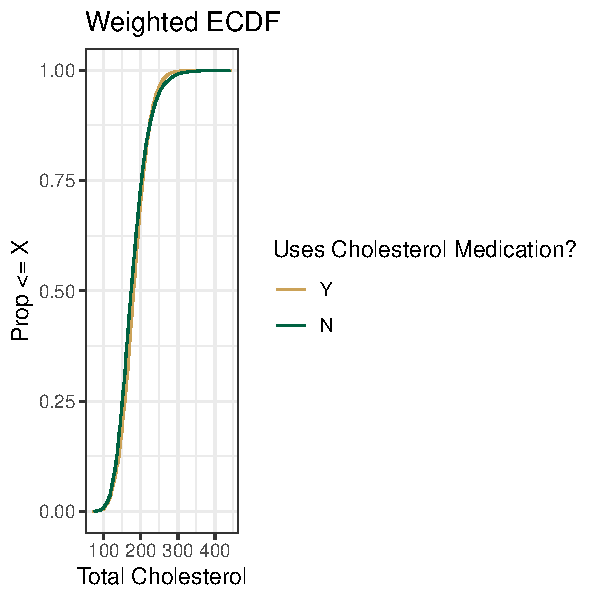
\includegraphics{final-project_files/figure-latex/fig_ecdf-1.pdf}
\caption{Empirical cummulative distribution function for numerical
covariates}
\end{figure}

\hypertarget{average-treatment-effect-among-the-treated}{%
\subsection{Average treatment effect among the
treated}\label{average-treatment-effect-among-the-treated}}

We estimated the average treatment effect of taking cholesterol-lowering
medication. Our findings indicate that, on average, individuals who take
cholesterol-lowering medication experience a decrease 3.911 mm Hg in
their Systolic Blood Pressure (SBP). We are 95 percent confident that
the average effect of taking this medication on SBP falls within the
range of at least -4.960 mm Hg to at most -2.863 mm Hg.

\begin{longtable}[]{@{}
  >{\raggedright\arraybackslash}p{(\columnwidth - 6\tabcolsep) * \real{0.5395}}
  >{\centering\arraybackslash}p{(\columnwidth - 6\tabcolsep) * \real{0.1316}}
  >{\centering\arraybackslash}p{(\columnwidth - 6\tabcolsep) * \real{0.1579}}
  >{\centering\arraybackslash}p{(\columnwidth - 6\tabcolsep) * \real{0.1711}}@{}}
\toprule()
\begin{minipage}[b]{\linewidth}\raggedright
\textbf{Characteristic}
\end{minipage} & \begin{minipage}[b]{\linewidth}\centering
\textbf{Beta}
\end{minipage} & \begin{minipage}[b]{\linewidth}\centering
\textbf{95\% CI}
\end{minipage} & \begin{minipage}[b]{\linewidth}\centering
\textbf{p-value}
\end{minipage} \\
\midrule()
\endhead
Taking a cholesterol-lowering medication & & & \\
No & --- & --- & \\
Yes & -3.9 & -5.0, -2.9 & \textless0.001 \\
\bottomrule()
\end{longtable}

\hypertarget{sensitivity-analysis}{%
\subsection{Sensitivity analysis}\label{sensitivity-analysis}}

We conducted a sensitivity analysis to account for the possibility that
our Directed Acyclic Graph (DAG) might not include all potential
confounding variables. In this analysis, we calculated the necessary
relationship between an unmeasured confounder and the change in weight
required to shift the lower bound of the confidence interval to the null
hypothesis level (5\%). We considered exposure confounder effects of
sizes 0.05, 0.10, and 0.15, which would necessitate confounder-outcome
effects of 172, 85, and 57, respectively, to influence the interval. The
smallest of these values, 57, is over 6 times greater than the estimated
treatment effect. Therefore, it is reasonable to conclude that the
Average Treatment Effect (ATT) we computed is robust against potential
confounding factors.

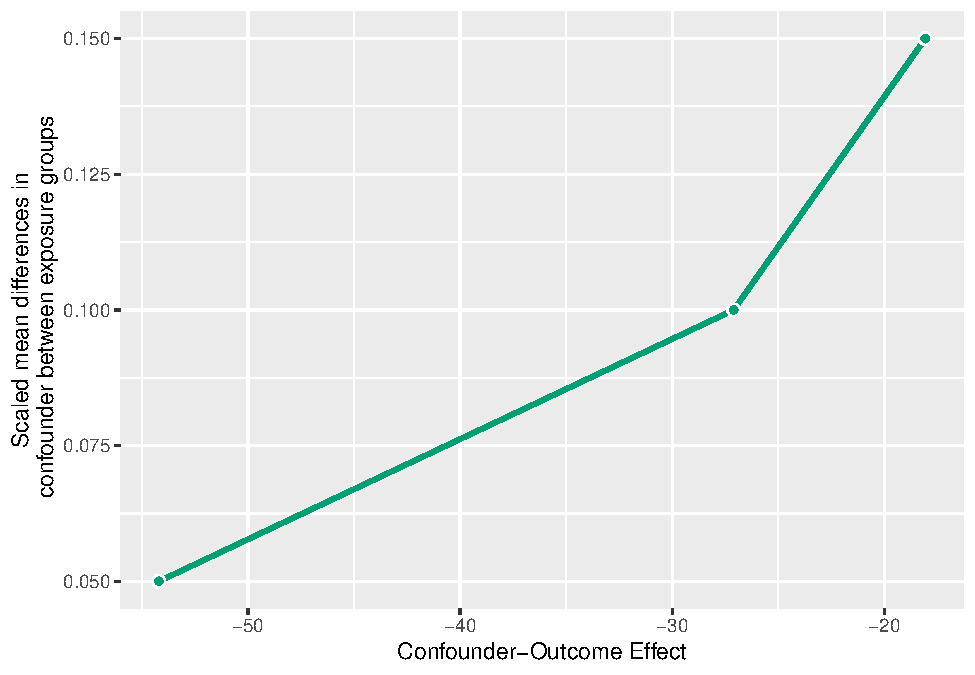
\includegraphics{final-project_files/figure-latex/tab_sensitivity-1.pdf}

\hypertarget{discussion}{%
\section{Discussion}\label{discussion}}

\hypertarget{limitation}{%
\subsection{Limitation}\label{limitation}}

Our dataset does not include information on when a person start taking
the anti-hypertensive medication and the cholesterol-lowering medication
in relation to a biophysical measurement.

Furthermore, in addition to pharmacotherapy, it is also important to
adopt a lifestyle change include exercise, a healthy diet, regulating
sodium, reducing alcohol use, reduce smoking, getting sleep, reducing
stress, and regular health check-ups.

Even with prescribed medication, the barriers to effective blood control
includes those that are under the control of the physician (patients'
insufficient education and motivation, reluctance to initiate lifestyle
changes or drug treatment) and those that are under the control of the
patients (failure to comply with recommended lifestyle modifications and
poor medication compliance) \citep{dusing_overcoming_2006}.

\hypertarget{conclusion}{%
\section{Conclusion}\label{conclusion}}

We conclude that for people taking cholesterol-lowering medication, they
should continue to do so.

\hypertarget{supplement}{%
\section{Supplementary information}\label{supplement}}

The data can be downloaded from GitHub or accessed via the
cardioStatsUSA R package. For both the file and information about the R
package, see \url{https://github.com/jhs-hwg/cardioStatsUSA}.

All code for the analysis can be accessed at \textbf{link github}

\hypertarget{acknowledge}{%
\section{Acknowledgement}\label{acknowledge}}

Thank Dr.~Lucy D'Agostino McGowan for her guidance and assistance in
preparing this manuscript.


\bibliographystyle{biom}
\bibliography{ref.bib}


\label{lastpage}


\end{document}
